\section{Problem Description}
This particular study seeks to formulate a method to design an equalizer beam using multi-objective optimization. To this end, an example system will be used as a subject for the design. The basic parameters for the solution are presented below. 

\section{Example System}
The example system to be studied is based on a few basic fixed design parameters. The basic outline of the beam structure is shown in Figure \ref{img:dim_beam}. 

\begin{figure}
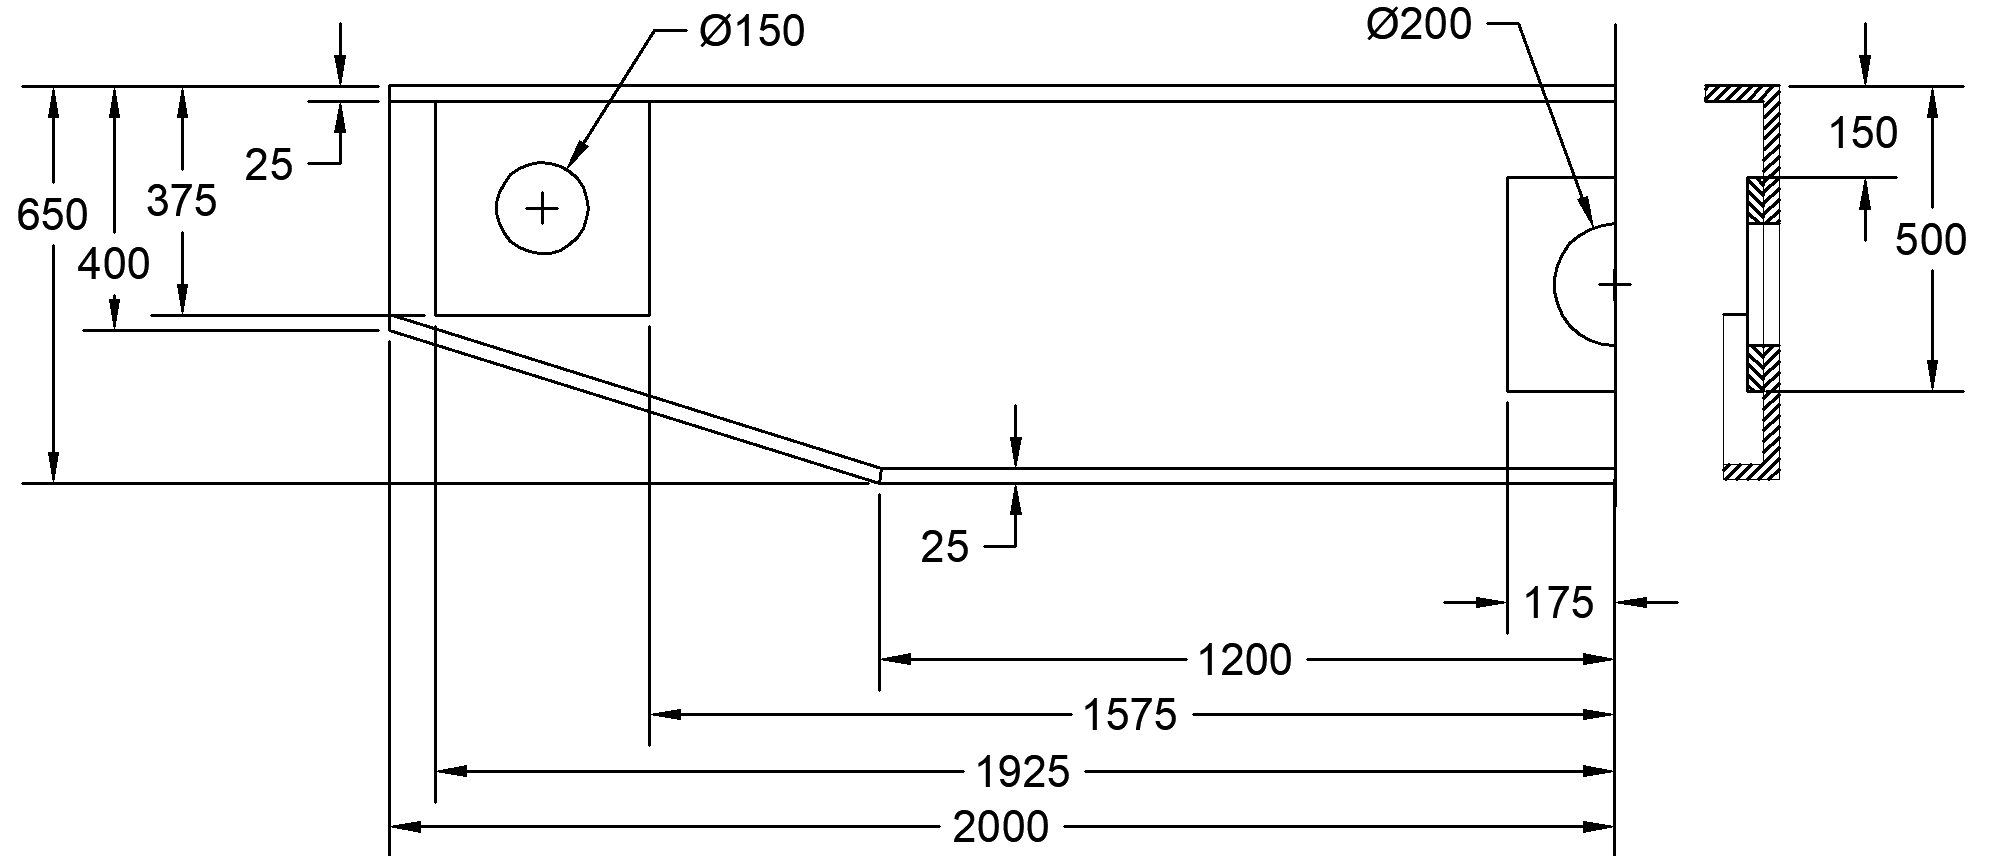
\includegraphics[width=\textwidth]{img/dim_beam.png}
	\label{img:dim_beam}
	\caption{Fixed Dimensions for the Example System Beam}
\end{figure}

Also fixed is the material, which is assumed to be ASTM A36 steel. The material has properties assumed to be: 

\begin{itemize}
\item Yield Strength: Mean 250MPa, Std. Deviation 32.5 MPa
\item Young's Modulus: 200 GPa
\end{itemize}

\subsection{Performance requirements}
In this case, performance requirements primarily relate to the lifting capacity and the allowable side pull on the beam. The requirements selected for this problem are: 
\begin{enumerate}
\item Lifting capacity: 60 metric tons, 60,000kg, 132,000 lbm, 588 kN. For this problem, 600 kN was used. 
\item Minimum capable side load: $\pm 5^{\circ} $
\end{enumerate}

As will be discussed in detail later, the beam to be analyzed is symmetric on 2 planes. This allows for the model to consist of only one quarter of the beam under study. Additionally, It will be later clarified that the selected solution methods utilize stochastic methods to model the loading. 
